\newpage
%
% Začiatok druhej časti analýzy
% Analýza podobných nástrojov
%
\ifthenelse {\boolean{bachelor}}
{
	%\section{Analysis}
	\section{Analýza podobných nástrojov} 
}
{
	%\chapter{Analysis}
	\chapter{Analýza podobných nástrojov}
}
Dostupnosť aplikácií na spracovanie prirodzeného jazyka je veľká a široká. Najväčší podiel tvoria aplikácie zamerané na preklad. My sa zameriame na aplikácie, ktoré umožňujú editovať paralelný text.

%
% Nástroje na správu paralelných textov
%
\ifthenelse {\boolean{bachelor}}
{
	%\section{Analysis}
	\subsection{Nástroje na správu paralelných textov} 
}
{
	%\chapter{Analysis}
	\section{Nástroje na správu paralelných textov}
}
Nástroje na správu paralelných textov uľahčujú spracovanie viacerých druhov a verzií textu. Na jednej strane majú zdrojový text alebo súbor a na druhej strane výsledný text alebo súbor. Hlavný dôraz sa kladie práve na transformáciu zo zdrojového textu na cieľový. Transformácia môže mať viacero podôb, ako preklad, zarovnanie alebo zjednodušenie textu, a mnoho ďalších. Texty sú zväčša rozdelené podľa viet, pre zjednodušenie transformácie, pričom vety na jednej úrovni zvyčajne spolu súvisia podľa určitej vlastnosti.

V následujúcich častiach si predstavíme niektorých predstaviteľov tohto druhu nástrojov.

%
% InterText
%
\ifthenelse {\boolean{bachelor}}
{
	%\subsection{Subsection}
	\subsection{InterText}
}
{
	%\section{Subsection}
	\section{InterText}
}
InterText\footnote{http://wanthalf.saga.cz/intertext} je editor paralelne zarovnaných textov, využívaný na správu viacerých paralelne zarovnaných verzií textu rôznych jazykov na úrovni viet. Táto aplikácia je dostupná vo verzií pre desktop, ale aj pre server.

Podporuje viacero formátovaní textu, či už čistý (angl. plain) text alebo XML a taktiž zobrazuje aj HTML značky. Riadky obsahujú vety oddelené znakom konca riadku a sú očíslované. Umožňuje funkcie ako presúvanie riadkov textu alebo zoskupenie viacerých do jedného, krok vpred a vzad. V spracovávanom texte sa dá vyhľadávať a je možné tento text aj upraviť podľa vlastných potrieb.

InterText nezohľadňuje používateľove úpravy textu počas používanie a pri následnom spracovávaní textu sa tak neprispôsobí používateľovi. Okrem toho zjednodušovanie textu v tomto nástroji by bolo pomerne náročné.

Na obrázku~\fullref{fig:intertext_interface} je zobrazená aplikácia InterText s testovacím vstupom, na ktorom je vidno väčšinu, už spomenutej, funkcionality, ako presúvanie a zoskupovanie riadkov, číslovanie, atď.

\begin{figure}[H]
	\begin{center}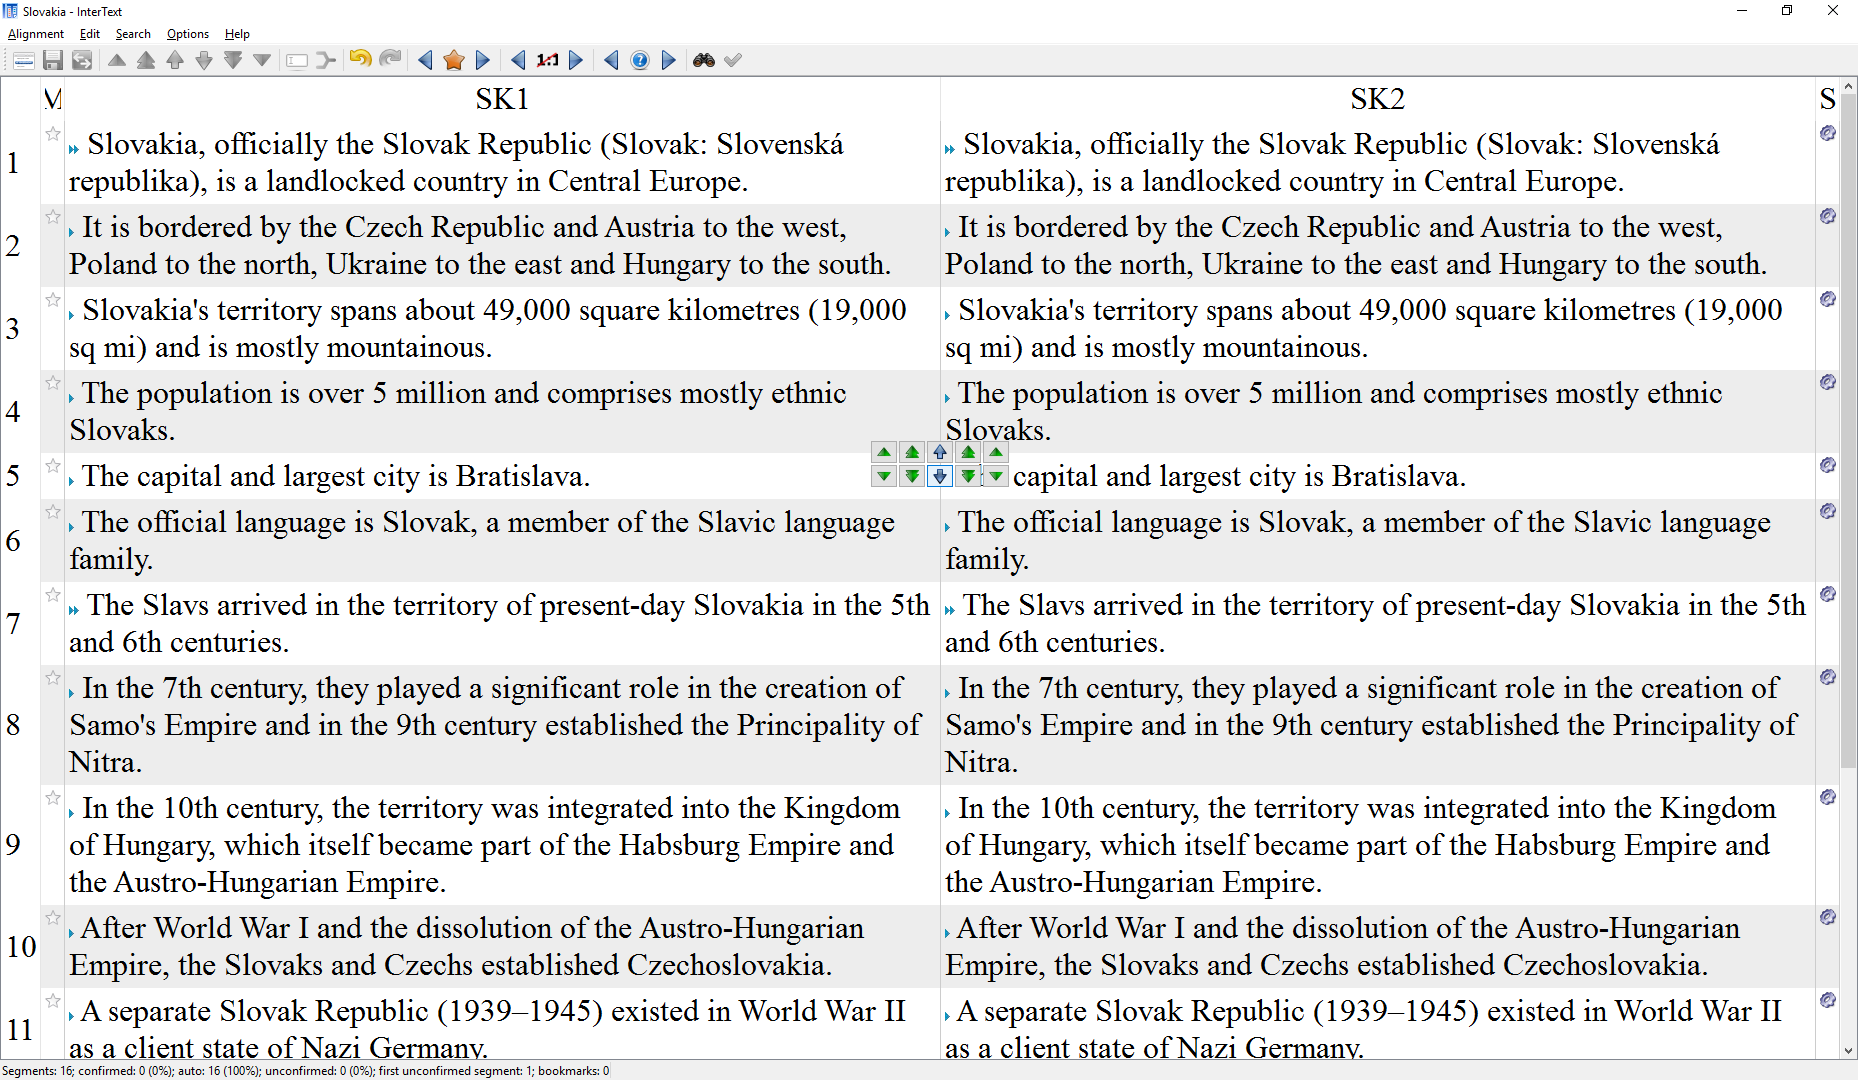
\includegraphics[scale=0.33]{intertext_interface}\end{center}
	\caption[Aplikácia InterText]{Aplikácia InterText}\label{fig:intertext_interface}
\end{figure}

%
% NOVA Text Aligner
%
\ifthenelse {\boolean{bachelor}}
{
	%\subsection{Subsection}
	\subsection{NOVA Text Aligner}
}
{
	%\section{Subsection}
	\section{NOVA Text Aligner}
}
NOVA Text Aligner\footnote{http://www.supernova-soft.com/wpsite/products/text-aligner/} je aplikácia na zarovnávanie textu, pričom nevyužíva algoritmy na zarovnávanie textu, ale manuálne používateľovo určovanie zarovnania.

Ako vidno na obrázku~\fullref{fig:nova_text_aligner_interface} hlavná editovacia časť aplikácie je rozdelené do dvoch častí. Umožňuje do ľavej aj pravej časti načítať rôzny text, v ktorom sa dá veľmi jednoducho vyhľadávať, k čomu napomáha zvýraznenie vyhľadaných slov. Načítaný text je možné premiestňovať a zoskupovať, či už podľa riadkov alebo aj v celých blokoch a nechýba možnosť editovať text. Je možné si túto aplikáciu prispôsobiť. Ponúka možnosti ako zmena typ písma a pod. Finálny, spracovaný text sa dá exportovať do viacerých formátov, z ktorých populárne sú formáty elektronických knižiek EPUB a MOBI.

Aplikácia je zameraná hlavne na usporadúvanie textu, nezaznamenáva si používateľove zmeny textu a neprispôsobuje sa podľa toho pri ďalšom použití, funguje iba lokálne. NOVA Text Aligner je dostupná iba v skúšobnej verzií, pre dlhodobé používanie si treba zakúpiť licenciu.

\begin{figure}[H]
	\begin{center}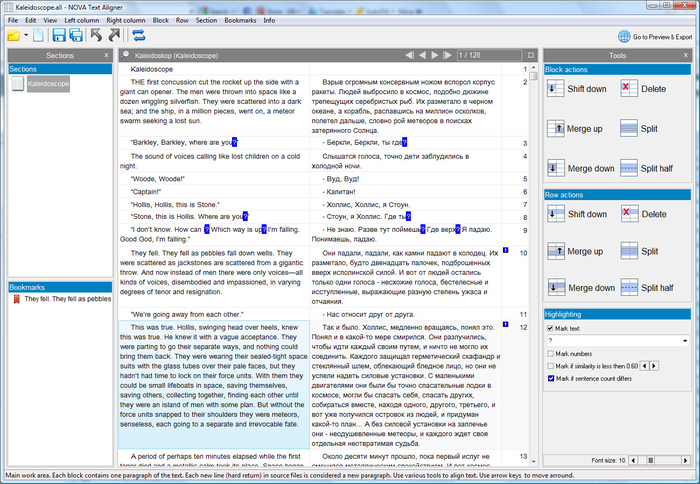
\includegraphics[scale=0.56]{nova_text_aligner_interface}\end{center}
	\caption[Aplikácia NOVA Text Aligner]{Aplikácia NOVA Text Aligner\footnotemark}\label{fig:nova_text_aligner_interface}
\end{figure}
\footnotetext{http://parallel-text-aligner.en.softonic.com/}

%
% LF Aligner
%
\ifthenelse {\boolean{bachelor}}
{
	%\subsection{Subsection}
	\subsection{LF Aligner}
}
{
	%\section{Subsection}
	\section{LF Aligner}
}
Aplikácia LF Aligner\footnote{www.sourceforge.net/projects/aligner} je zameraná na spracovanie textu rôznych jazykov. Ponúka možnosť použiť až 99 jazykov, čo ale znamená 99 vstupných súborov, každý so zvoleným jazykom. Dokáže spracovať rôzne typy vstupných súborov od čistého textu, PDF súborov, cez URL stránok s textom až po správy Európskeho parlamentu, ktoré automaticky stiahne. Výstup môže byť taktiež viacerých druhov, napríklad cez grafické rozhranie LF Aligner alebo vygenerovanie XLS súboru. Na obrázku~\fullref{fig:lf_aligner_interface} vidno grafické rozhranie tejto aplikácie, ktoré ponúka mnohé vymoženosti. Samozrejmosťou je možnosť premiestňovať a zoskupovať riadky, doplnenie ďalšieho súboru na spracovávanie, uloženie zmien súboru prepísaním jeho dát a mnohé ďalšie.

\begin{figure}[H]
	\begin{center}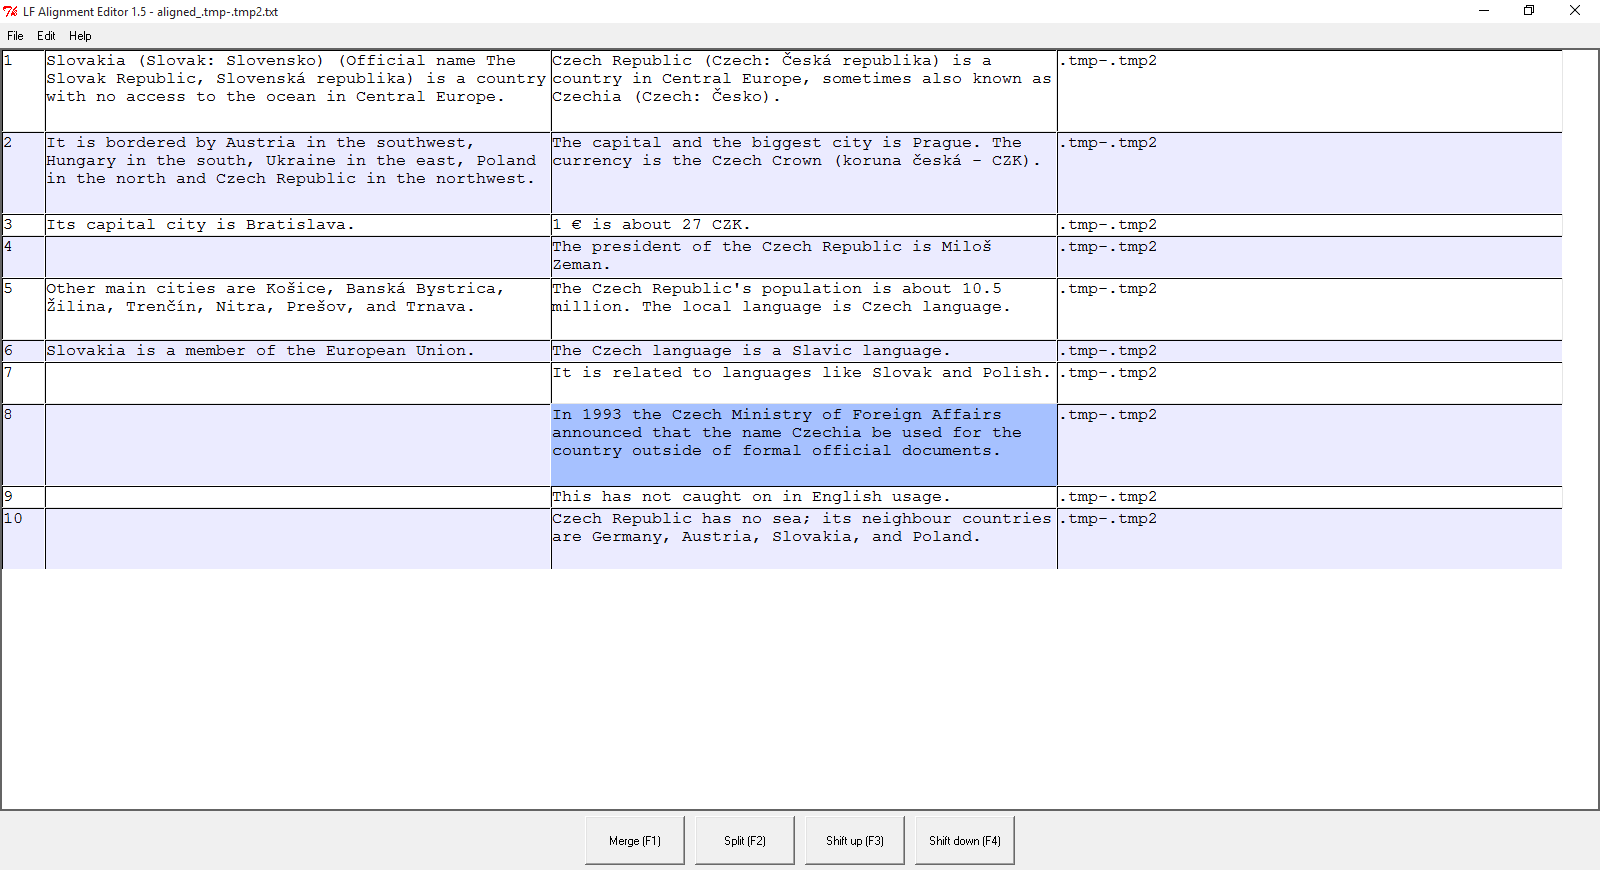
\includegraphics[scale=0.33]{lf_aligner_interface}\end{center}
	\caption[Aplikácia LF Aligner]{Aplikácia LF Aligner}\label{fig:lf_aligner_interface}
\end{figure}
\footnotetext{http://parallel-text-aligner.en.softonic.com/}

%
% Google Translate
%
\ifthenelse {\boolean{bachelor}}
{
	%\subsection{Subsection}
	\subsection{Google Translate}
}
{
	%\section{Subsection}
	\section{Google Translate}
}
Za najznámejšieho zástupcu webových nástrojov na spracovanie paralelných textov sa dá pokladať nástroj Google Translate\footnote{translate.google.com}. Využíva sa na preklad slov, viet, ale dokáže spracovať aj celé texty. Momentálne podporuje preklad z a do 91 jazykov. Dokáže rozpoznať a preložiť hovorenú reč aj písaný text. Pri preklade jednotlivých slov zobrazuje viacero možných prekladov do druhého jazyka, pričom pri preklade z anglického jazyka ponúka aj ukážky viet, v ktorých sa prekladané slovo môže použiť. Správnu výslovnosť preloženého aj prekladaného slova alebo textu, si používateľ môže vypočuť na krátkej zvukovej ukážke.

Na obrázku~\fullref{fig:google_translate_example} je zobrazený preklad anglického textu do slovenského. Vidno, že preklad do minoritných jazykov ešte nie je dokonalý.

\begin{figure}[H]
	\begin{center}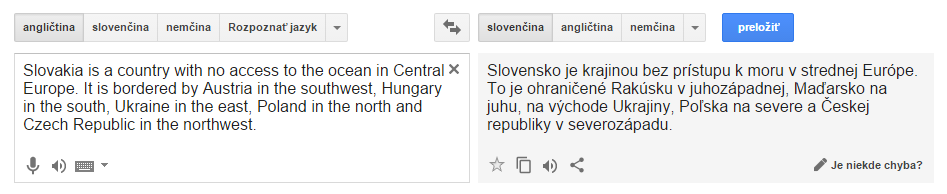
\includegraphics[scale=0.55]{google_translate_example}\end{center}
	\caption[Google Translate]{Google Translate}\label{fig:google_translate_example}
\end{figure}

%
% Zhrnutie aplikácií na spracovanie prirodzeného jazyka
%
\ifthenelse {\boolean{bachelor}}
{
	%\subsection{Subsection}
	\subsection{Zhrnutie}
}
{
	%\section{Subsection}
	\section{Zhrnutie}
}
Analyzovali sme aplikácie, ktoré umožňujú spravovať a editovať paralelný text. Za ich pomoci dokážeme zo vstupného textu získať výstupný text. Napríklad pri preklade máme vstupný text množinu viet v anglickom jazyku, ktorú chceme preložiť do slovenského jazyka a výstupný text je preloženú množinu viet. Pri zjednodušovaní textu je na vstupe taktiež množina viet a na výstupe je každá veta zo vstupnej množiny zjednodušená podľa istých pravidiel. Výstupný text vzniká určitou transformáciou vstupného textu, aplikovaním transformácie na každú vetu zdrojového textu.

Analyzované nástroje nespĺňajú všetky požiadavky na systém schopný spoznámkovať učebný text v takom rozsahu, ktorý by umožňoval používateľovi prispôsobiť si spracovaný text. Systém musí umožňovať editáciu jednotlivých viet výstupného textu podľa vôle používateľa. Tieto úpravy musí zohľadniť pri následnej aplikácií transformácií vstupného textu. Takisto musí ukladať dáta mimo používateľovho úložného priestoru.

%
% Smerovanie práce
%
\ifthenelse {\boolean{bachelor}}
{
	%\section{Analysis}
	\section{Smerovanie práce} 
}
{
	%\chapter{Analysis}
	\chapter{Smerovanie práce}
}
V letnom semestri plánujem najskôr dokončiť prototyp. To znamená, spraviť používateľské rozhranie, ktoré bude umožňovať vložiť text na spracovanie, zobrazí poznámky a tak isto umožní používateľovi pre ľubovolnú vetu pozmeniť tvar poznámky poznámky. Tieto zmeny sa uložia do databázy a zohľadnia pri ďalšom použití. Úprava spracovanej poznámky bude fungovať na princípe preusporiadania slov vety, takže používateľ nebude môcť zadať kadečo. Predíde sa tým nezmyselným záznamom v databáze.

Do systému doimplementovať ,,AND poznámkovač'', ktorý identifikuje množinu súvisiacu so spojkou AND a pre každú entitu v tejto množine oddelenú čiarkou vygeneruje samostatnú poznámku.

Následne plánujem dokončiť kapitolu návrh, napísať kapitoly závar, anotácia, výsledky a ďalšie.
%
% Opis prototypu
%
\ifthenelse {\boolean{bachelor}}
{
	%\section{Analysis}
	\section{Opis prototypu} 
}
{
	%\chapter{Analysis}
	\chapter{Opis prototypu}
}
V zimnom semestri som implementoval prototyp aplikácie na spoznámkovanie učebného textu.

%
% Notenizer
%
\ifthenelse {\boolean{bachelor}}
{
	%\section{Analysis}
	\subsection{Notenizer} 
}
{
	%\chapter{Analysis}
	\section{Notenizer}
}
\label{subsection:notenizer}
\textbf{Notenizer} je prototyp aplikácie na extrahovanie relevantných informácií z učebných textov. Využíva nástroj Stanford CoreNLP, ktorý je implementovaný v Jave, ale cez IKVM je portnutý aj na C\#. Na ukážke \fullref{code:spustenie_stanford_corenlp} je ukázané prepojenie nástroja StanfordCoreNLP s aplikáciou Notenizer. 
\\

\begin{lstlisting}[ language = csharp, caption={Spustenie StanfordCoreNLP}, label = {code:spustenie_stanford_corenlp}]
String jarRoot = @"stanford-corenlp-3.5.2-models";

Properties properties = new Properties();
// Zvolime, ktore nastroje chceme pouzit.
// pos = part-of-speech tagger
// ssplit = sentence split
// atd.
properties.setProperty("annotators", "tokenize, ssplit, pos, parse");
properties.setProperty("sutime.binders", "0");
properties.setProperty("ner.useSUTime", "false");

// Nastavenie aktualneho priecinku, aby StanfordCoreNLP vedel najst
// vsetky potrebne subory
String currentDirectory = Environment.CurrentDirectory;
Directory.SetCurrentDirectory(jarRoot);
StanfordCoreNLP pipeline = new StanfordCoreNLP(properties);
Directory.SetCurrentDirectory(currentDirectory);

// Vytvorenie anotacie z textu
Annotation annotation = new Annotation(text);

// Spustenie
pipeline.annotate(annotation);
\end{lstlisting}

Údaje získane z tohto nástroja, napríklad POS značky, vzťahy medzi slovami, pozície slov a mnoho ďalších, Notenizer ďalej spracováva. Najdôležitejšie vlastnosti, ktoré sa využívajú v najväčšej miere pri spracovávaní sú závislosti (angl. dependency) medzi slovami vo vete.  

Spracovávaný text sa postupne spracováva po vetách. Každá veta sa samostatne ,,rozparsuje'', spoznámkuje. Vety sa parsujú na základe pravidiel. Na začiatku je daná statická sada pravidiel na spracovanie viet a textov. Po tom, ako sa celý text spracuje, tak sa použité pravidlá uložia do databázy aj s informáciami o pôvodnej vete a novo vytvorenej, zjednodušenej vete. Následne pri opätovnom používaní aplikácie, keď sa začne spracovávať text, tak sa vyhľadajú pre každú vetu pravidlá v databáze, vyberú sa tie s najväčšou zhodou a podľa toho sa spracuje daná veta. Statické pravidla na spracovanie vety sa v tomto prípade použijú len v prípade, ak v sa v databáze nenašli žiadne pravidlá na spracovanie vety, ktoré by pre danú vetu vyhovovali, to znamená, že takúto alebo podobnú vetu zatiaľ Notenizer nespracovával.

Na obrázku~\fullref{fig:example_output} je ukázaný ukážkový výstup prototypu pre vstupný text z wikipédie:
\textit{Czech Republic (Czech: Česká republika) is a country in Central Europe, sometimes also known as Czechia (Czech: Česko). The capital and the biggest city is Prague. The currency is the Czech Crown (koruna česká - CZK). 1€ is about 27 CZK. The president of the Czech Republic is Miloš Zeman. The Czech Republic's population is about 10.5 million. The local language is Czech language. The Czech language is a Slavic language. It is related to languages like Slovak and Polish. In 1993 the Czech Ministry of Foreign Affairs announced that the name Czechia be used for the country outside of formal official documents. This has not caught on in English usage. Czech Republic has no sea; its neighbour countries are Germany, Austria, Slovakia, and Poland.}
\\

Výstup je v tvare [pôvodná veta] ===>> [poznámka z pôvodnej vety].

\begin{figure}[H]
	\begin{center}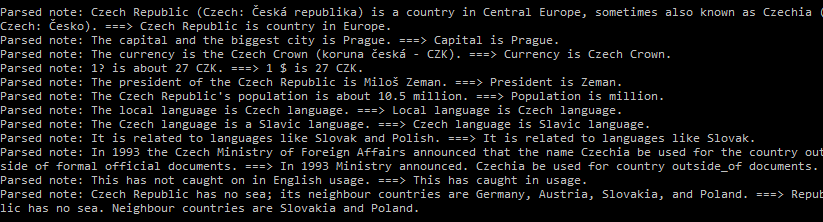
\includegraphics[scale=0.7]{example_output}\end{center}
	\caption[Ukážkový výstup prototypu]{Ukážkový výstup prototypu}\label{fig:example_output}
\end{figure}

%
% Pravidlá
%
\ifthenelse {\boolean{bachelor}}
{
	%\subsection{Subsection}
	\subsubsection{Pravidlá}
}
{
	%\section{Subsection}
	\subsection{Pravidlá}
}
\label{subsubsec:notenizer_pravidla}
Pri spracovaní pôvodnej vety sa na túto vetu aplikuje \textit{pravidlo na spracovanie}. Toto pravidlo obsahuje okrem iného zoznam závislostí pôvodnej vety. Podľa týchto závislostí slov vo vete sa v spracovávanej vete vyhľadajú slová, ktoré majú byť použité v poznámke. Vyhľadávajú sa, okrem iného, podľa POS značiek a indexov vo vete. Pre podrobnejšie informácie o vyhľadávaní a vytváraní pravidiel viď. sekcie~\fullref{subsubsection:rule_lookup} a~\fullref{subsubsection:rule_creation}

Obsahuje aj zoznam závislostí zjednodušenej vety, poznámky. Tieto závislosti sa aplikujú na spracovávané vety na vygenerovanie zjednodušenej vety (viď.~\fullref{subsubsection:rule_application}).